%!TEX root = ../../thesis.tex
\section{Components}

The implementation of XBMCMagic was an experiment to write as less JavaScript code as possible and to use AngularJS's expressions\todo{link to expressions description} wherever it was possible. Most frontend code has been achieved by solely using expressions, built-in directives and lean controllers which mostly act as glue code to services or third party libraries.

\subsection{Controllers}

\begin{figure}[htb]
  \centerline{
    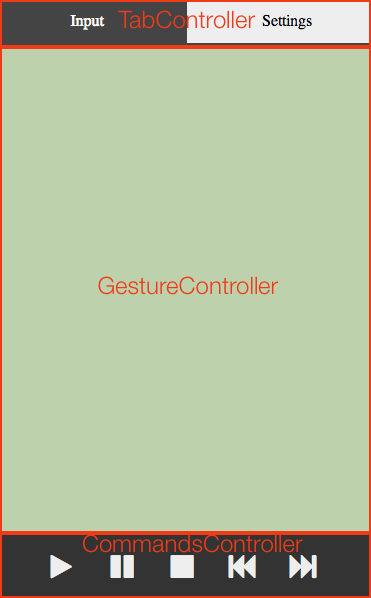
\includegraphics[width=0.4\linewidth]{images/xbmc-magic-screen-1.png}
    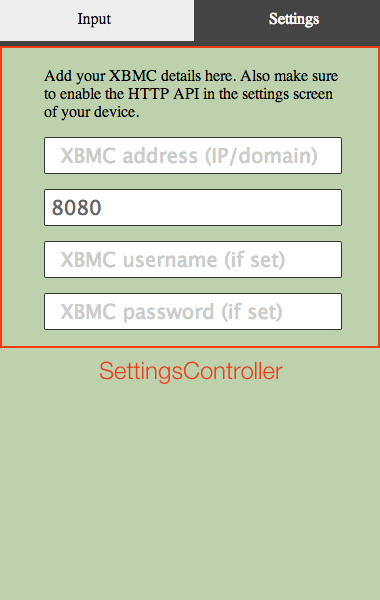
\includegraphics[width=0.41\linewidth]{images/xbmc-magic-screen-2.png}
  }
  \caption[left: initial screen, right: settings screen]{left: initial screen, right: settings screen}
  \label{fig:xbmcmagic-controllers}
\end{figure}

The app consists of only four controllers which are shown in \reffigure{fig:xbmcmagic-controllers}:

\subsubsection{TabController}

The TabController takes care of switching the currently visible tab and consists only of expressions in the template and one line of JavaScript in the controller file itself (\code{\$scope.currentTab = 0}). The controller is registered in the first line of \reflisting{lst:tab-controller} and from then on the logic relies entirely on directives and expressions. Line 9 switches (\code{ng-switch}) the shown content tab based on the value of \code{currentTab}, which is changed on click (\code{ng-click}) on one of the tab headers in line 3 or in line 6. Furthermore, the visual state of a tab header is changed according to the state of \code{currentTab} as well by using the \code{ng-class} directive.

\begin{lstlisting}[language=HTML, caption=TabController expressions, label=lst:tab-controller]
  <div class="tabs" ng-controller="TabController">
    <div class="tab-header">
        <div  ng-class="{`active': currentTab == 0}"
              ng-click="currentTab = 0">Input</div>

        <div  ng-class="{`active': currentTab == 1}"
              ng-click="currentTab = 1">Settings</div>
    </div>
    <div ng-switch="currentTab">
      <div ng-switch-when="0"><!-- GESTURES --></div>
      <div ng-switch-when="1"><!-- SETTINGS --></div>
    </div>
  </div>
\end{lstlisting}

\subsubsection{GestureController}



\subsubsection{CommandsController}

\subsubsection{SettingsController}

\subsection{Services}

\subsubsection{SettingsController}